\chapter{Einleitung}
\label{sec:Einleitung}

\section{Das Projekt}
%------------------------------------------------------------------------------------------------------------------------------
\subsection{Ausgangslage} \index{Ausgangslage}
Aus den ersten beiden Studienjahren haben wir uns die Grundkenntnisse der Java-Programmierung angeeignet
Wir m�chten dieses Wissen nutzen, um ein neues Gebiet zu betreten (Native-App Android) und uns einem Thema zu widmen, das uns interessiert, wir aber bis anhin keine Zeit gefunden haben.
Keiner von uns hat berufliche Programmiererfahrung. Deshalb liegt all unsere Erfahrung auf den schulischen Kenntnissen.


%------------------------------------------------------------------------------------------------------------------------------
\subsection{Ziel der Arbeit} \index{Ziel der Arbeit}
Unser prim�res Ziel ist es, einen Einblick in die Programmierung von Android Apps zu haben.
Zus�tzlich m�chten wir unser bereits angeeignetes Java-Wissen auffrischen und vertiefen





%------------------------------------------------------------------------------------------------------------------------------
\subsection{Aufgabenstellung} \index{Aufgabenstellung}
Wir m�chten eine Android App erstellen, die es dem User erm�glicht Garantiescheine in Form von einem Foto lokal auf dem Smartphone zu verwalten. Das App soll die M�glichkeit bieten, zus�tzliche Details in Form von Text zu speichern.
Da im Fokus vor allem der Einblick in die App- Programmierung steht, verzichten wir bewusst g�nzlich auf Netzwerk-Unterst�tzung. 
Des Weiteren ist das Backup der Fotos sowie der dazugeh�rigen Details nicht Teil dieser Arbeit, da dies unsere Zeitlimiten �bersteigen w�rde.

%------------------------------------------------------------------------------------------------------------------------------
\newpage
\subsection{Erwartetes Resultat} \label{subsec:erwartetesResultat}
Das erwartete Resultat ist ein Native-App, welches auf Android funktioniert. Folgende Anforderungen m�ssen erf�llt sein.

\begin{itemize} 
\item Kein Absturz der Applikation
\item Lauff�hig auf Ger�ten mit OS $>2.2$ (Froyo) bis hin zum aktuellen 4.1.x (Jelly Bean) 
\item Fotos k�nnen aufgenommen und lokal gespeichert werden
\item Es k�nnen Details in Form von Freitext zu den Fotos hinzugef�gt werden
\item Garantiescheine sollen nach folgenden Kriterien sortiert werden k�nnen
		\begin{itemize}
		\item Speicherdatum des Garantiescheins
		\item Alphabetisch nach Titel
		\item Anzahl Tage bis Garantie ausl�uft
		 \end{itemize}
 \end{itemize}


%------------------------------------------------------------------------------------------------------------------------------
\subsection{Geplante Termine}


\begin{table}[h!]
\begin{minipage}{10cm}
\caption{geplante Termine}
\label{tab:geplante_Termine}
\begin{tabular}[t]{|l|l|} \hline
 \cellcolor{darkgrey} &  \cellcolor{darkgrey}  \\ 
\cellcolor{darkgrey} \multirow{-2}{3cm}{\textbf{Datum}} &
\cellcolor{darkgrey} \multirow{-2}{6cm}{\textbf{Beschreibung}}  \\  \cline{1-2}
3 Oktober 2012 & Einschreiben des Projektes im EBS  \\ \cline{1-2}
5. Dezember 2012 & Abgabe Teaser im EBS \\ \cline{1-2}
12. Dezember 2012 & Arbeitstreffen \\   \cline{1-2}
9. Januar 2013 & Abgabe der Dokumentation \\  \cline{1-2}
16. Januar 2013 & Pr�sentation \\  \cline{1-2}
\end{tabular}

\end{minipage}
\end{table}



%------------------------------------------------------------------------------------------------------------------------------
\newpage
\subsection{Teaser}
\index{Teaser}
Am 5. Dezember 2012 musste per Mail ein Teaser abgegeben werden.\\

\textbf{Definition Teaser gem�ss Wikipedia:}\\
\textit{Ein Teaser (von engl. tease = reizen, necken) ist in der Werbesprache ein kurzes Text- oder Bildelement, das zum Weiterlesen, -h�ren, -sehen, -klicken verleiten soll.}\\

Da das Ziel eines Teaser ist, den Leser zur Applikation zu verleiten, sollte der Teaser auch die Applikation widerspiegeln.
Aus diesem Grund wurde der Teaser bewusst ganz schlicht gehalten, genau so wie die daraus resultierende Applikation.\\

\begin{figure}[h!]
\centering
\fbox{
\noindent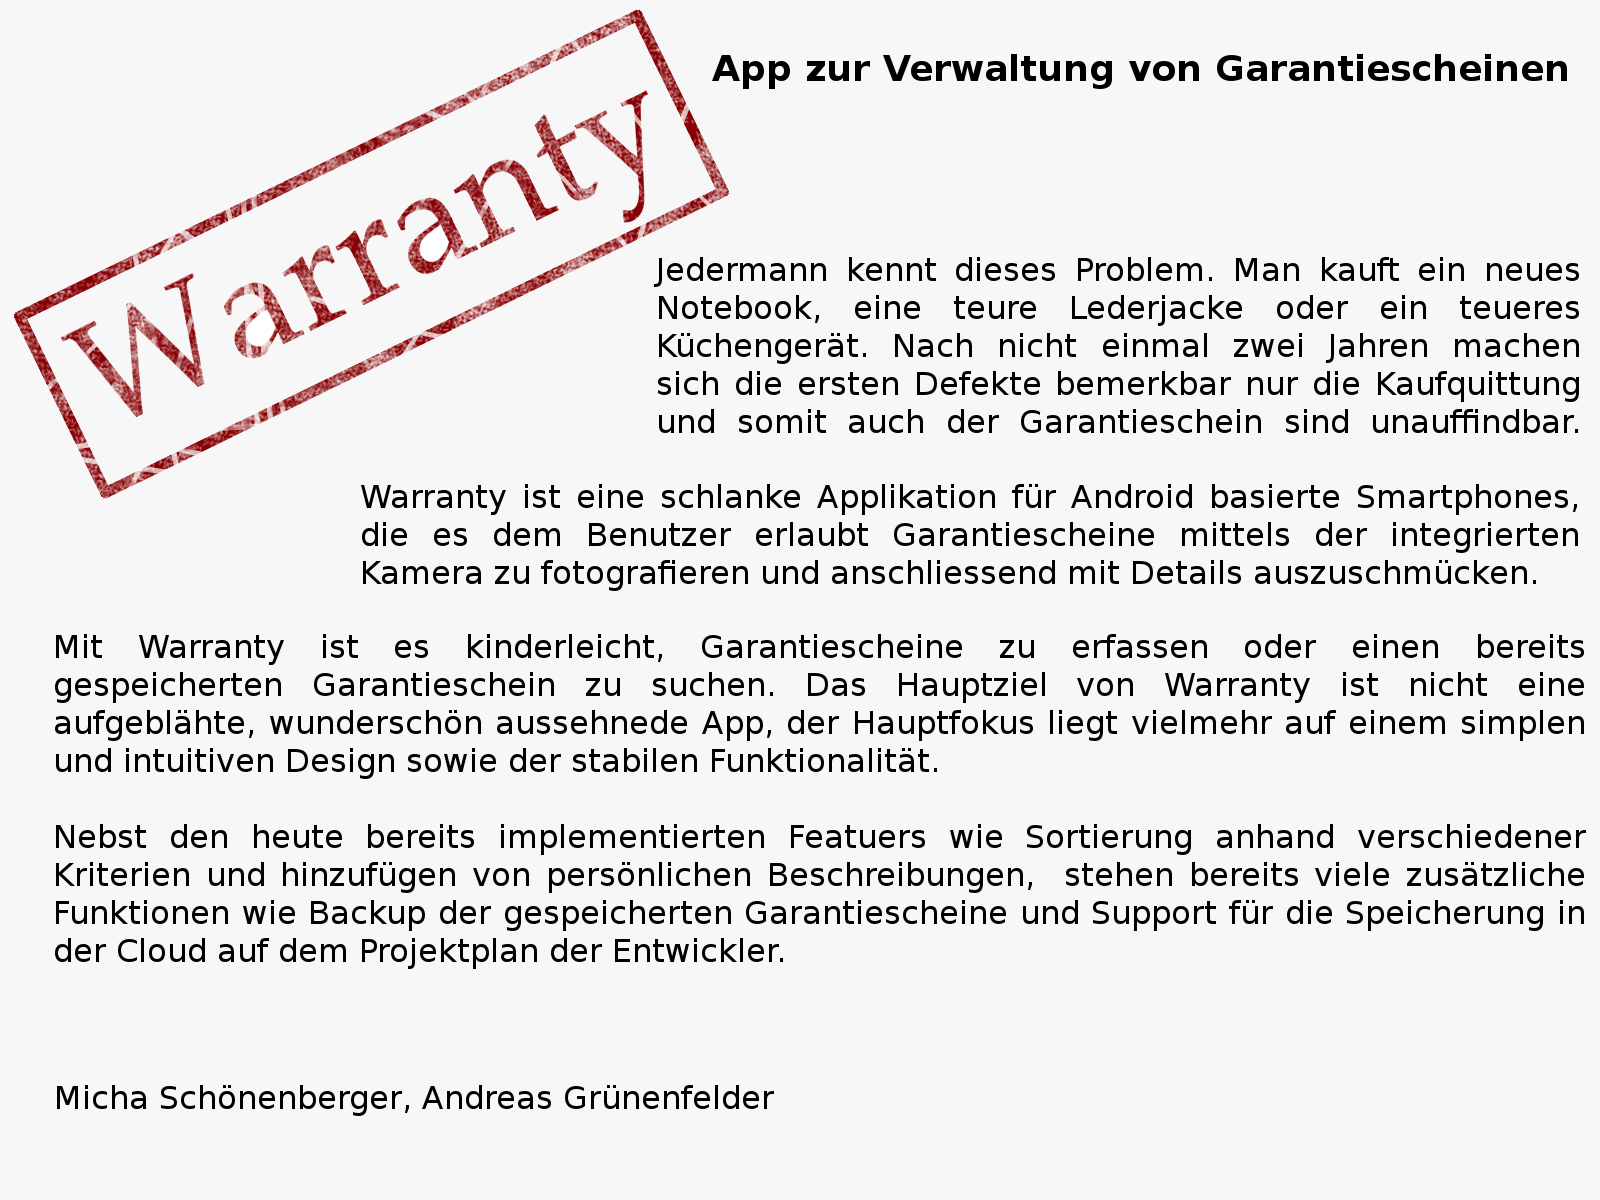
\includegraphics[width=\textwidth]{warranty_teaser.png} }

\caption{abgegebener Teaser (05. Dezember 2012)}
\label{fig:Teaser}
\end{figure}





